\documentclass[sigconf]{acmart}
\usepackage{amsmath}
\usepackage{graphicx}
\graphicspath{{./images/}}
\usepackage{caption}
\usepackage{subcaption}
\usepackage[notransparent]{svg}
\usepackage{hyperref}  % Added for hyperlink support


% Meta information
\title{Image “Outpainting” and Hole Filling: Final Report}
\subtitle{CS 5787 Deep Learning Final Project Report}

\author{Wentao Ye}
\email{wy335@cornell.edu}
\affiliation{%
  \institution{Cornell University}
  \city{New York}
  \state{New York}
  \country{USA}
}

\author{Mitchell Krieger}
\email{mak483@cornell.edu}
\affiliation{%
  \institution{Cornell University}
  \city{New York}
  \state{New York}
  \country{USA}
}

\author{Sebastian Jay}
\email{srj63@cornell.edu}
\affiliation{%
  \institution{Cornell University}
  \city{New York}
  \state{New York}
  \country{USA}
}

% Document begins
\begin{document}

\maketitle

\section*{Team Members}
Wentao Ye (wy335), Mitchell Krieger (mak483), Sebastian Jay (srj63)

\section*{Introduction}
This paper explores the relationship between image inpainting and outpainting by training a model capable of interpolating between two disparate images, blending them seamlessly into a single coherent scene. Inpainting, or image interpolation, is a computer vision task that aims to fill in missing or removed sections of an image, ensuring the completed area integrates smoothly with the existing content. Outpainting, or image extrapolation, generates extensions of an image beyond its original borders.

Drawing inspiration from both inpainting and outpainting, our objective is to generate a transitional region between two images. Traditional inpainting requires an understanding of the context and semantics surrounding the missing area to blend edges seamlessly into the original image. Outpainting, while sharing these challenges, has less context to infer from since it involves extending the image into an unknown space. Additionally, outpainting must handle long-range semantic dependencies, ensuring the generated extensions remain consistent with the original image no matter how far the extrapolation extends. Our task incorporates these challenges and introduces an added complexity: the need for the generated region to be semantically consistent with both images.

\section*{Related Work}
To address the challenges of our task, we leverage deep learning architectures capable of capturing both the semantics at the edges of each image and the relationships between regions across the two images. Historically, Convolutional Neural Networks (CNNs) have been widely used in vision tasks due to their efficiency and ability to learn spatial relationships \cite{LeCun1998, Krizhevsky2012}. However, CNNs have inherent limitations stemming from their design. Their architecture emphasizes locality, with weight sharing across the entire input, which makes them less adept at capturing long-range dependencies or relationships between non-local regions—a key requirement for complex tasks like ours.

Transformer-based architectures, particularly those employing attention mechanisms, have shown effectiveness in both inpainting and outpainting due to their capacity to model long-range dependencies. For example, \cite{Jiahui2018} demonstrated that incorporating a contextual attention layer significantly improved inpainting performance. Vision Transformers (ViTs) introduced by \cite{Dosovitskiy2020} expanded on this by applying self-attention mechanisms to computer vision tasks, enabling the modeling of global relationships in an image. Further advancements, such as Swin Transformers \cite{Liu2021}, refined the transformer architecture for vision tasks using hierarchical computation and shifted windows to improve efficiency and adaptability. These approaches, however, remain computationally expensive and require large datasets for effective training \cite{Dascoli2021}.

Yang et al. (2019) proposed a U-net GAN architecture to perform very long outpainting of a scene in one direction. They used Skip Horizontal Connections to connect each layer of the encoder and decoder in the Unet and an LSTM-based Recurrent Transfer Network to transfer the encoded sequences to the decoder. Using this method and generating in multiple steps, they were able to demonstrate long outpainting. Lu et al. (2021) expanded on this work by combining inpainting, outpainting, and image blending to fill in a scene between two images horizontally. They introduced a similar U-net GAN architecture to Yang et al. but also incorporated contextual attention and a Bidirectional Content Transfer module, which used LSTMs as a bottleneck to ensure spatial and semantic consistency across two images. Our work generalizes this approach by extending it to painting between two images in multiple directions.

\section*{Datasets}
We used the \textcolor{red}{\href{https://github.com/z-x-yang/NS-Outpainting}{NS-Outpainting}} dataset to train our models. It is used in the original U-Transformer paper. We also tested our trained model on additional images sourced from the internet.

\section*{Methods}
\subsection*{Architecture}
Our approach employs a Generative Adversarial Network (GAN) framework that integrates a U-Net-based generator and a PatchGAN-based discriminator. We chose these architectures to effectively handle the challenges of our interpolation task. Specifically, the generator is responsible for synthesizing the transitional region between two input images, producing outputs that not only blend these images seamlessly but also remain contextually and semantically consistent. The discriminator, on the other hand, aims to distinguish real, fully integrated images from those generated by the model, thereby guiding the generator toward more authentic and coherent results.

\subsubsection*{Generator (U-Net)}
The generator in our framework is inspired by the U-Net architecture, originally proposed by Ronneberger et al. (2015). U-Net is known for its encoder-decoder structure with symmetric skip connections that allow spatial details lost in downsampling operations to be reintroduced at corresponding upsampling stages. This architectural feature is crucial for high-resolution image synthesis tasks, such as ours, because it helps preserve both low-level details (e.g., textures and edges) and high-level semantic cues that are essential for coherent blending. The U-Net generator consists of a series of downsampling convolutional layers that progressively capture increasingly abstract features. These encoder stages are followed by a bottleneck layer and a series of corresponding upsampling layers that reconstruct the image back to the original resolution. Skip connections transfer feature maps from the encoder to the decoder, ensuring that spatial and contextual information is retained throughout the synthesis process. The final layer of the generator uses a Tanh activation function to constrain the output pixels to the [-1, 1] range, consistent with our input normalization scheme. This U-Net variant has been successfully applied in tasks like inpainting and outpainting, thus making it a suitable choice for our image interpolation objective.

\subsubsection*{Discriminator (PatchGAN)}
Instead of a standard discriminator that outputs a single scalar probability for the entire image, we adopt a PatchGAN-based discriminator \cite{Isola2017}. The PatchGAN discriminator classifies overlapping local patches of the image as real or fake, rather than the entire image at once. This approach has shown effectiveness in encouraging finer local detail synthesis and prevents the generator from focusing solely on global consistency. By examining smaller regions independently, the PatchGAN discriminator ensures that textures, edges, and local structures are faithfully rendered, ultimately contributing to more realistic intermediate regions.

\begin{figure}[h!]
    \centering
    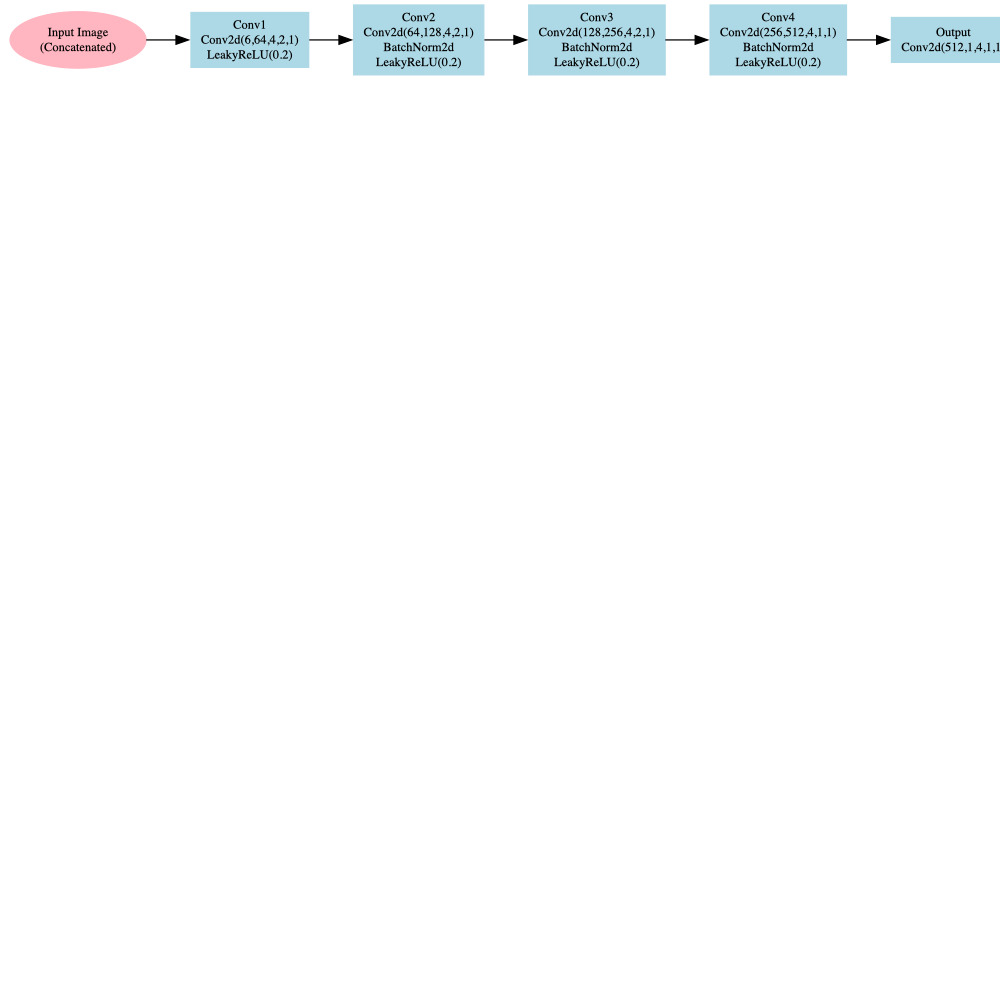
\includegraphics[width=\linewidth]{discriminator}
    \caption{Illustration of the U-Net discriminator architecture.}
    \label{fig:discriminator}
\end{figure}

\subsection*{Training Procedure}
Our GAN is trained in an adversarial manner. The generator \( G \) takes as input a partially masked image that combines two cropped regions—one from the left-bottom portion of one scene and one from the right-top portion of another scene—thus producing a coherent output that fills in the missing portions. The discriminator \( D \) is trained to distinguish the ground-truth combined scene from the generated ones. Throughout training, \( G \) aims to produce outputs that are indistinguishable from real images, while \( D \) refines its ability to detect generated content, pushing \( G \) to create more realistic and semantically consistent results.

\subsection*{Loss Functions}
\textbf{Adversarial Loss:}

We employ a standard least-squares GAN objective for the adversarial training (Mao et al., 2017). For the discriminator, the loss compares real and fake patches, encouraging it to assign a high score to real imagery and a low score to generated content. The generator, conversely, seeks to produce patches that the discriminator deems real.

\textbf{Reconstruction Loss (L1 Loss):}

To ensure that the generated content closely matches the ground-truth target image in the masked regions, we use an L1 reconstruction loss:

\textbf{Structural Similarity (SSIM) Loss:}

While pixel-level losses help guide low-level detail, we also incorporate a Structural Similarity Index (SSIM) loss to ensure perceptual quality and to maintain local image structures. The SSIM-based term computes how structurally similar the generated region is to the target, adding a complementary metric that focuses on luminance, contrast, and structural attributes

\textbf{Perceptual Loss:}

Inspired by style transfer and inpainting literature, we include a perceptual loss derived from pre-trained VGG-19 features (Johnson et al., 2016). This loss compares high-level representations of the generated and ground-truth images

\textbf{Combined Objective:}

The total generator loss is a weighted combination of these terms:
\[
\mathcal{L}_{G} = \mathcal{L}_{\text{GAN}}(G,D) + \lambda_{\text{recon}}\mathcal{L}_{\text{recon}}(G) + \lambda_{\text{SSIM}}\mathcal{L}_{\text{SSIM}}(G) + \lambda_{\text{perc}}\mathcal{L}_{\text{perc}}(G),
\]


\subsection*{Implementation Details}

Our implementation uses PyTorch, and we normalize inputs to the $[-1, 1]$ range. The models are trained using the Adam optimizer (Kingma \& Ba, 2015) with a learning rate of $2 \times 10^{-4}$ and $\beta_1 = 0.5$, $\beta_2 = 0.999$. We periodically save model checkpoints and evaluate intermediate outputs to ensure that the generator’s outputs become progressively more realistic and semantically meaningful. 

By combining the strengths of the U-Net generator, PatchGAN discriminator, and multiple complementary loss functions, our method is able to learn complex inter-image relationships and produce visually and contextually coherent transitions between two given images. The following sections detail our experimental setup and results, demonstrating the effectiveness of this approach in bridging visually distinct images into a single, harmonious scene.

\section*{Experiments}

\subsection*{Experimentation Steps}

We completed the following steps when experimenting on our models, sometimes stopping early and not completing all steps if we did not see comparable results to our previous work:

\begin{enumerate}
    \item \textbf{Training:} As explained above, we removed the upper right and lower left quadrants of each training image and computed loss metrics on the model’s prediction of the original intact image without any quadrants removed. We then computed metrics on the test set by evaluating the model’s prediction of the uncropped test set images, using cropped test set images with their upper right and lower left quadrants removed as input.
    
    \item \textbf{Visual inspection of results on the same cropped input image:} Before computing metrics, we visually inspected each model’s outputs when computing predictions from the test set. When this step yielded low or unrecognizable resemblance to the input image, we stopped and revised the model.
    
    \item \textbf{Metrics computation:} We computed the Peak Signal-to-Noise (PSNR), Structural Similarity Index Measure (SSIM), and Fréchet Inception Distance (FID) metrics for each model on the test images.
    
    \item \textbf{Visual inspection of results on two different cropped input images:} In contrast to step 2, where we used two quadrants of the same image, here we used the upper right quadrant of one image and the lower left quadrant of a different image as input to the model and visually inspected the resulting completed image of an intact scene.
    
    \item \textbf{Visual inspection with larger cropping mask of one input image:} Here we repeated step 2, but instead of using the entire lower left quadrant and the entire upper right quadrant as input (which meet at the center of the image), we only used the bottom left portion of the lower left quadrant and the upper right portion of the upper right quadrant, which do not meet in any part of the image.
    
    \item \textbf{Visual inspection with larger cropping mask of two different images:} Here we used a larger mask as in step 5 on two distinct images of different scenes, as in step 4.
\end{enumerate}

We trained and tested all of our models on the NS-Outpainting dataset containing wide panoramic images of scenery. Some example images from it are shown below:

\begin{figure}[h!]
    \centering
    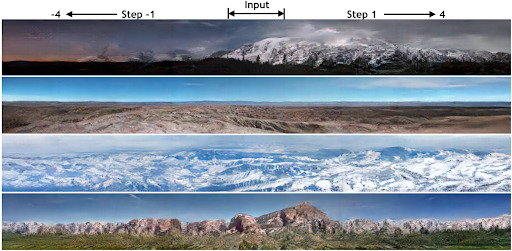
\includegraphics[width=\linewidth]{ns_dataset}
    \caption{Example images from the NS-Outpainting dataset that we used to train our models.}
    \label{fig:ns_dataset}
\end{figure}

\subsection*{Models}

We experimented with the following models:

U-Transformer model: here we sought to replicate the results achieved by Gao et al in the “Generalised Image Outpainting with U-Transformer” paper. We completed experimentation steps 1-2 for this model as a reference point, but found that achieving results comparable to that of the paper was computationally infeasible with our resources.

\begin{figure}[h!]
    \centering
    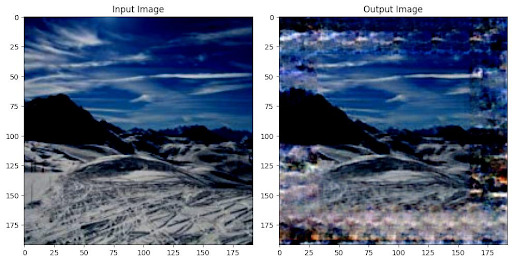
\includegraphics[width=\linewidth]{u_transformer}
    \caption{Output from the U-Transformer model, to paint outwards from the original image. Note that this is not the same task as we are attempting to complete with our models.}
    \label{fig:u_transformer}
\end{figure}

The first diffusion model that we tried was inspired by the “Repaint” diffusion model published by Lugmayr et al in the paper “RePaint: Inpainting using Denoising Diffusion Probabilistic Models”. The architecture is shown here:

\begin{figure}[h!]
    \centering
    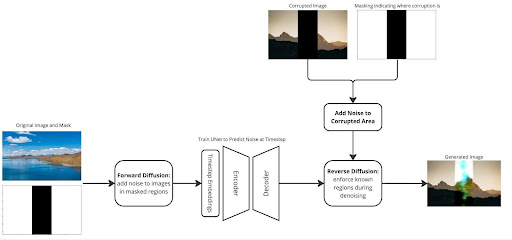
\includegraphics[width=\linewidth]{repaint_architecture}
    \caption{Illustration of our model's architecture that was based on the RePaint diffusion model architecture.}
    \label{fig:repaint_architecture}
\end{figure}

And our output from using this model is shown below:

\begin{figure}[h!]
    \centering
    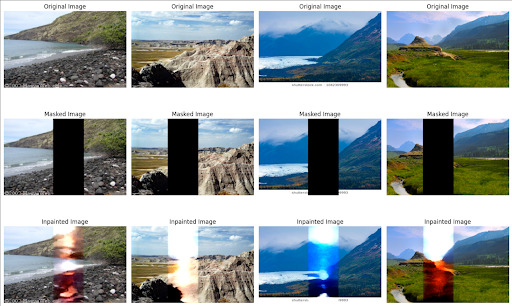
\includegraphics[width=\linewidth]{repaint_results}
    \caption{Output from the RePaint model that we tried.}
    \label{fig:repaint_results}
\end{figure}

However, we realized after producing these output images that there was some leakage from the training data into the test data. Hence, we do not consider this to be a valid result.

Our best independently developed result was achieved with our GAN model, which uses the PatchGAN discriminator and UNet generator as described in greater detail above. Our GAN model’s architecture is shown below, showing an example raw input image, cropped input image, and generated output image:

\begin{figure}[h!]
    \centering
    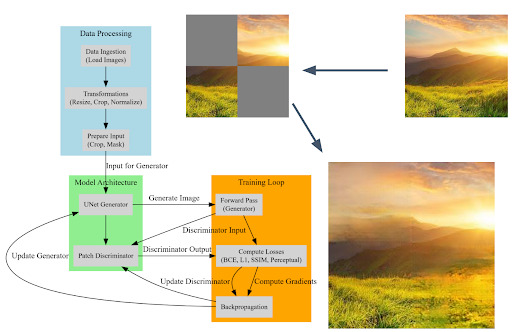
\includegraphics[width=\linewidth]{gan_architecture}
    \caption{Architecture of our final GAN model.}
    \label{fig:gan_architecture}
\end{figure}

Below are some of the results that we achieved using the GAN model on our test set of images, when the model received one cropped image of the same scene as input (i.e. step 2 in the list of “Experimentation Steps” above):

\begin{figure}[h!]
    \centering
    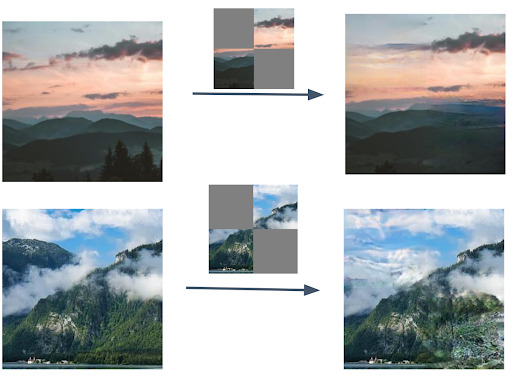
\includegraphics[width=\linewidth]{gan_step_2}
    \caption{Results from experimentation step 2 of our final GAN model}
    \label{fig:gan_step_2}
\end{figure}

Here are the metrics that we achieved with our GAN model, using the outputs from step 2 in our list of “Experimentation Steps” above:

\begin{figure}[h!]
    \centering
    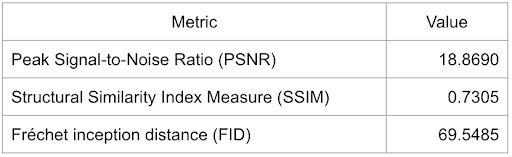
\includegraphics[width=\linewidth]{gan_metrics}
    \caption{Metrics achieved by our final GAN model on the test set of images, as described in experimentation step 2.}
    \label{fig:gan_metrics}
\end{figure}

Below are some of the results that we achieved using the GAN model on our test set of images, when the model received two adjacent and distinct images of different scenes as input, each cropped to only contain one quadrant (i.e. step 4 in the list of “Experimentation Steps” above):

\begin{figure}[h!]
    \centering
    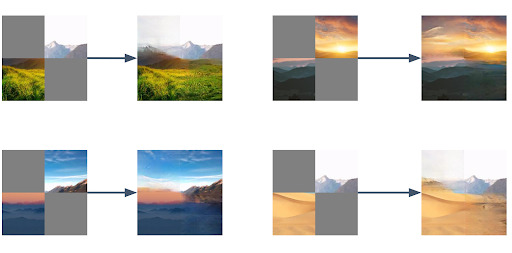
\includegraphics[width=\linewidth]{gan_step_4}
    \caption{Results outputted by our final GAN model from input images of two separate scenes, as described in experimentation step 4.}
    \label{fig:gan_step_4}
\end{figure}

We tried repeatedly to train a non-pretrained diffusion model from scratch but were unable to achieve visually satisfactory results with it. Here are some examples of what it produced in step 2:

\begin{figure}[h!]
    \centering
    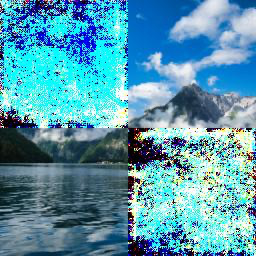
\includegraphics[width=\linewidth]{diffusion_step_2_1}
    \caption{Example 1: our non-pretrained diffusion model output from Experimentation Step 2.}
    \label{fig:diffusion_step_2_1}
\end{figure}

\begin{figure}[h!]
    \centering
    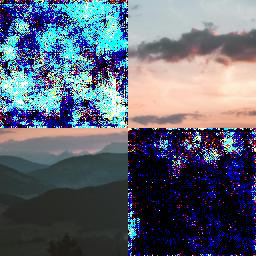
\includegraphics[width=\linewidth]{diffusion_step_2_2}
    \caption{Example 2: our non-pretrained diffusion model output from Experimentation Step 2.}
    \label{fig:diffusion_step_2_2}
\end{figure}

\begin{figure}[h!]
    \centering
    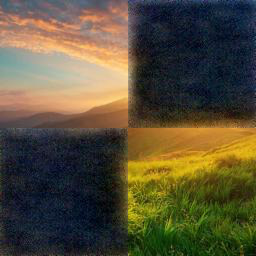
\includegraphics[width=\linewidth]{diffusion_step_2_3}
    \caption{Example 3: our non-pretrained diffusion model output from Experimentation Step 2.}
    \label{fig:diffusion_step_2_3}
\end{figure}

\begin{figure}[h!]
    \centering
    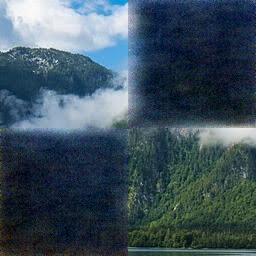
\includegraphics[width=\linewidth]{diffusion_step_2_4}
    \caption{Example 4: our non-pretrained diffusion model output from Experimentation Step 2.}
    \label{fig:diffusion_step_2_4}
\end{figure}

\begin{figure}[h!]
    \centering
    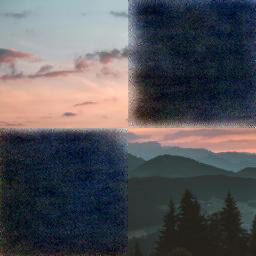
\includegraphics[width=\linewidth]{diffusion_step_2_5}
    \caption{Example 5: our non-pretrained diffusion model output from Experimentation Step 2.}
    \label{fig:diffusion_step_2_5}
\end{figure}

Finally, here are some of the results that we achieved using the GAN model on our test set of images, when the model received two non-adjacent distinct images of different scenes as input, each cropped more extensively to contain only part of one quadrant (i.e. step 6 in the list of “Experimentation Steps” above):

\begin{figure}[h!]
    \centering
    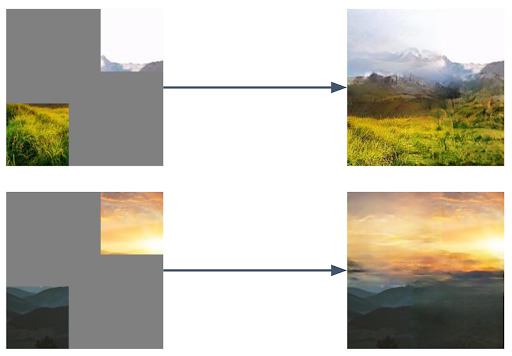
\includegraphics[width=\linewidth]{gan_step_6}
    \caption{Our final GAN model's output in experimentation step 6, using non-adjacent images of disparate scenes.}
    \label{fig:gan_step_6}
\end{figure}

As a comparison benchmark, we also tried a pre-trained Stable Diffusion model from huggingface. Example results from steps 2 and 5 are shown below:

\begin{figure}[h!]
    \centering
    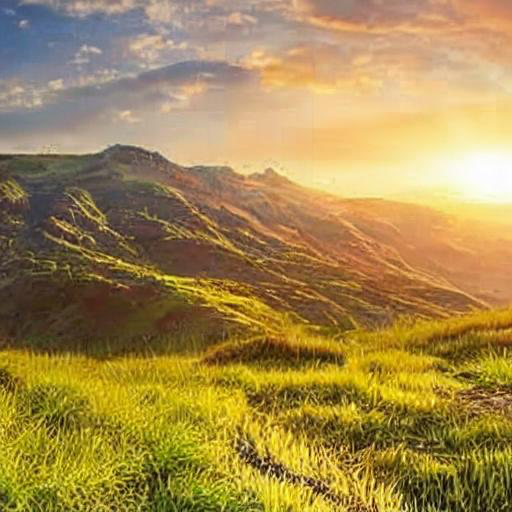
\includegraphics[width=\linewidth]{stable_diffusion_step_2_1}
    \caption{Example 1: pretrained Stable Diffusion model output from Experimentation Step 2.}
    \label{fig:stable_diffusion_step_2_1}
\end{figure}

\begin{figure}[h!]
    \centering
    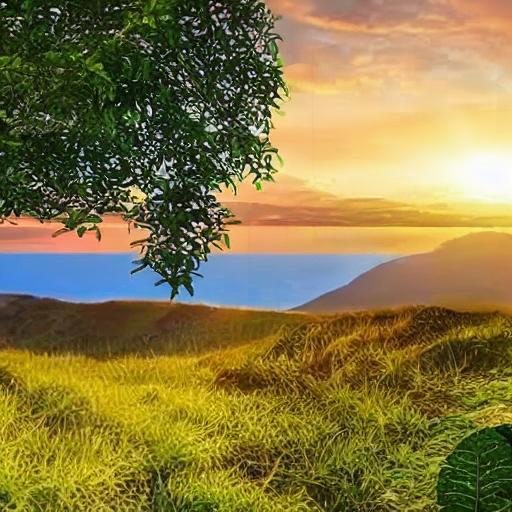
\includegraphics[width=\linewidth]{stable_diffusion_step_2_2}
    \caption{Example 2: pretrained Stable Diffusion model output from Experimentation Step 2.}
    \label{fig:stable_diffusion_step_2_2}
\end{figure}

\begin{figure}[h!]
    \centering
    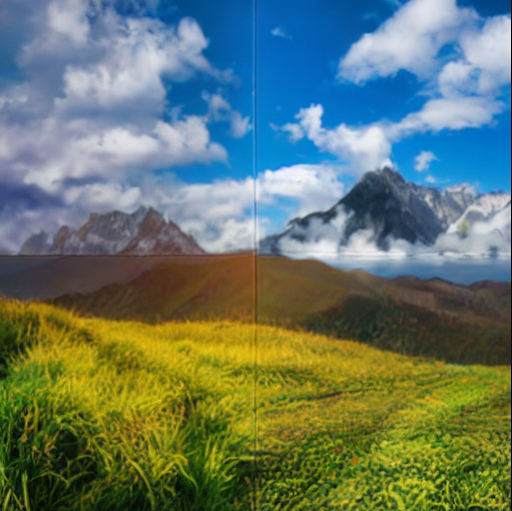
\includegraphics[width=\linewidth]{stable_diffusion_step_5}
    \caption{Example 1: pretrained Stable Diffusion model output from Experimentation Step 5.}
    \label{fig:stable_diffusion_step_5}
\end{figure}

\section*{Conclusion}

As can be seen from the images above, the best results that we achieved from a model that we developed were obtained from our final GAN model, which integrates a U-Net-based generator and a PatchGAN-based discriminator.

Notably, the state of the art pretrained Stable Diffusion model \textit{“was trained using 256 Nvidia A100 GPUs on Amazon Web Services for a total of 150,000 GPU-hours, at a cost of \$600,000.”} By contrast, we achieved the results shown above with our GAN model after training for just 5 hours on a RTX 2070. We’d love to see what our final GAN model can achieve with a training budget of \$600,000!

\section*{Appendix}

All of our code can be found in \textcolor{red}{\href{https://github.com/yewentao256/CS5787-Final}{our repository}} on Github.

\begin{thebibliography}{9}
    \bibitem{Dascoli2021} Stéphane d’Ascoli et al., "ConViT: Improving Vision Transformers with Soft Convolutional Inductive Biases," \textit{CVPR 2021}, 2021.
    \bibitem{Dosovitskiy2020} A. Dosovitskiy, et al., "Discriminative Unsupervised Feature Learning with Exemplar Convolutional Neural Networks," \textit{IEEE Transactions on Pattern Analysis and Machine Intelligence}, 2020.
    \bibitem{Gao2022} Penglei Gao et al., "Generalised Image Outpainting with U-Transformer," \textit{CVPR 2022}.
    \bibitem{Isola2017} P. Isola, et al., "Image-to-Image Translation with Conditional Adversarial Networks," \textit{CVPR 2017}.
    \bibitem{Jiahui2018} J. Yang, et al., "Contextual Attention for Image Inpainting," \textit{CVPR 2018}.
    \bibitem{Krizhevsky2012} A. Krizhevsky, et al., "ImageNet Classification with Deep Convolutional Neural Networks," \textit{NIPS 2012}.
    \bibitem{LeCun1998} Y. LeCun, et al., "Gradient-Based Learning Applied to Document Recognition," \textit{Proceedings of the IEEE}.
    \bibitem{Liu2021} Z. Liu, et al., "Swin Transformer: Hierarchical Vision Transformer Using Shifted Windows," \textit{ICCV 2021}.
    \bibitem{Lu2021} Chia-Ni Liu, et al., "Bridging the Visual Gap: Wide-Range Image Blending," \textit{CVPR 2021}.
    \bibitem{Lugmayr2022} Andreas Lugmayr, et al., "RePaint: Inpainting Using Denoising Diffusion Probabilistic Models," \textit{CVPR 2022}.
    \bibitem{Mao2017} X. Mao, et al., "Least Squares Generative Adversarial Networks," \textit{ICCV 2017}.
    \bibitem{Mostaque2022} @EMostaque on Twitter, "The Stable Diffusion model was trained using 256 Nvidia A100 GPUs on Amazon Web Services for a total of 150,000 GPU-hours, at a cost of \$600,000." \textit{https://twitter.com/EMostaque/status/1509780730730734592}
    \bibitem{Rombach2022} Robin Rombach, et al., "High-Resolution Image Synthesis with Latent Diffusion Models," \textit{CVPR 2022}.
    \bibitem{Tang2024} Luming Tang, et al., "RealFill: Reference-Driven Generation for Authentic Image Completion," \textit{SIGGRAPH 2024}.
    \bibitem{Yang2019} Zongxin Yang, et al., "Very Long Natural Scenery Image Prediction by Outpainting," \textit{ICCV 2019}.
    \bibitem{Yu2018} Jiahui Yu et al., "Generative Image Inpainting with Contextual Attention," \textit{CVPR 2018}.
\end{thebibliography}

\end{document}
